% #region PREAMBEL OG PAKKER
\documentclass[a4paper, 12pt]{article}  % DOKUMENTKLASSE
\title{Eksamen ØKO1001\\Del 1: Ledelse} % TITTEL
\author{Kandidatnr. 10026}              % FORFATTER
\date{\today}                           % DATO & FAG

\usepackage[english, norsk]{babel}      % NORSK SPRÅK
\usepackage[                            % BIBLIOGRAFI
    backend=biber,
    style=apa,
    ]{biblatex}
\usepackage{csquotes}                   % PAKKE TIL BABEL
\addbibresource{ref.bib}                % PATH TIL BIBLIOGRAFI
\usepackage[hidelinks]{hyperref}        % LENKER I TOC OG GENERELT
\usepackage[margin=1in]{geometry}       % VANLIG STØRRELSE MARGIN
\setlength{\parindent}{0em}             % SKILLER AVSNITT
\setlength{\parskip}{1em}               % SKILLER AVSNITT
\usepackage{setspace}
\setstretch{1.4}                        % 1.5 LINJEAVSTAND
\usepackage{graphicx}                   % BILDER \includegraphics[OPTIONS]{PATH}
\usepackage{kantlipsum}                 % FYLLTEKST I KANT-STIL (kant[n-m])
\usepackage{amsfonts}                   % BLACKBOARD BOLD FONT (\mathbb{N})
\usepackage{import}                     % IMPORTER FILER (\import{PATH}{FILE})
\usepackage{caption}                    % PAKKE FOR BEDRE CAPTIONS I FIGURER
\usepackage{float}                      % FLYTT FIGURER 
\usepackage{booktabs, multirow} % for borders and merged ranges
\usepackage{soul}% for underlines
\usepackage[table]{xcolor} % for cell colors
\usepackage{changepage,threeparttable} % for wide tables
% #endregion
\begin{document}
% #region INNHOLDSFORTEGNELSE
\maketitle
\vfill
\begin{center}
  ØKO1001 - Ledelse
\end{center}
\thispagestyle{empty}
\addtocounter{page}{-1}
\newpage
\tableofcontents % INNHOLDSFORTEGNELSE
\thispagestyle{empty}
\addtocounter{page}{-1}
% #endregion
\newpage
\section{Quiet quitting og ledelse?}

\subsection{Hva er <<Quiet quitting>>?}

Quiet quitting er en trend fra USA som har spredt seg som ild i tørt gress i sosiale medier, og særlig på plattformen TikTok. 
Ifølge Bergens Tidene har emneknaggen \texttt{\#quietquitting} over 274 millioner treff på TikTok \parencite{bt22}, og fenomenet har også tatt veien til Norge. 
Quiet quitting går kort fortalt ut på at man som arbeidstaker ønsker å ha et klart og tydelig skille mellom arbeid og fritid, 
<<\emph{Gjør jobben din, å dra hjem}>> omtaler Sigrid Sollund det som i Dagsnytt 18 \parencite{dax18}.

Fenomenet er populær bland generasjon Z, unge arbeidstakere født fra slutten av 90-tallet til rundt 2010, 
og det er kanskje også derfor den florerer på sosiale medier i de plattformene de unge brukes mest.
Det er derimot ikke bare de unge som følger trenden. 
I følge amerikansk gallup er halvparten av de ansatte i USA såkalte quiet quitters \parencite{dax18}.

Det ironiske med quiet quitting er nettopp det at det har sitt utspring fra USA; landet der man skal kunne få til alt man vil. 
Den amerikanske drømmen går ut på at hvem som helst kan få til hva som helst, så lenge man jobber hardt nok. 
Amerikaneren Frank Sinatra sier det best selv <<\emph{If I can make it there, I'll make it anywhere}>>. 
Tar man quiet quitting på kornet kan det heller minne om Aksel Sandemoses Jantelov, <<\emph{Du skal ikke tro at du \emph{er} noe}>>, og kanskje er det derfor det også har slått ann i Norge.

\subsection{Er Quiet quitting et problem for ledere?}

1000kr spørsmålet er da om dette er et problem for lederne? 
Trenger de i det hele tatt å bry seg om at alle ikke vil legge inn det lille ekstra, og gi litt mer innsats enn de trenger? 
Vel, det kan avhenge veldig ut i fra hva slags leder man er. 
Hvis vi tar utgangspunkt i Blake og Moutons \emph{ledergitter} (Figur \ref{fig:ledergitter}) ser vi rammeverket for fem forskjellige ledere.

Alle disse fem ledertypene vil ha et anderledes forhold til en quiet quitter. 
La oss starte med å ta utgangspunkt i ledertypen nederst til venstre i gitteret, <<\emph{La-det-skure}>>-lederen.

\begin{figure}[H]
  \centering
  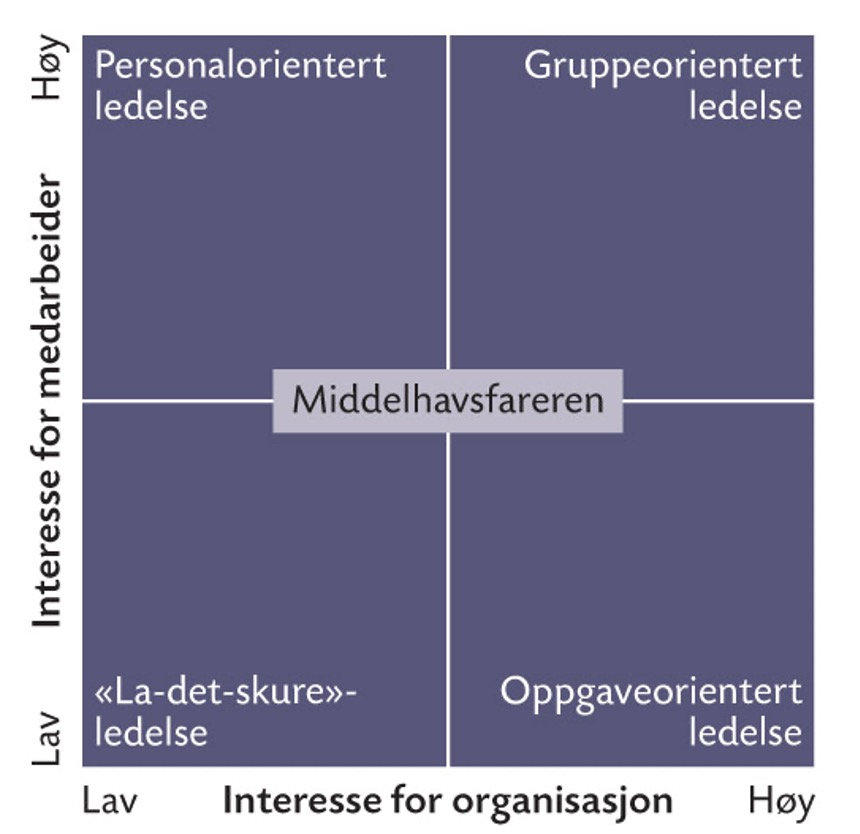
\includegraphics[width=8cm]{img/ledergitteret.jpg}
  \caption{Ledergitteret \parencite[63]{ledelse}}
  \label{fig:ledergitter}
\end{figure}

En leder som følger \emph{<<La-det-skure>>-ledelse} vil neppe føle noen store problemer eller utfordringer med en quiet quitter. 
Lederen bryr seg nemlig i praksis lite om medarbeiderne og like lite om bedriftens resultater \parencite{ledelse}. 
At en medarbeider bare gjør akkurat det de blir bedt om og ikke noe mer er jo midt i blinken! 
<<Hva skal jeg si, du gjør jo akkurat det du får beskjed om, hva annet kan jeg forvente!>> kan man tenke seg lederen vil si under en medarbeidersamtale.

Den rake motsetningen finner vi ikke overraskende i motsatt felt i gitteret, den \emph{gruppeorienterte} lederen; 
en leder som er veldig motivert til å oppnå gode resultater, og motivere sine medarbeidere. 
Her kan det oppstå store gnister under en medarbeidersamtale med en quiet quitter. 
Lederen kan oppfatte medarbeideren som lat og uinteressert, og medarbeideren kan oppfatte lederen som påtrengende og slitsom.

I samme båt, men på hver sin ende, finner vi den \emph{personalorienterte} og den \emph{oppgaveorienterte} lederen. 
Disse lederne vil oppleve liknende utfordringer som den gruppeorienterte lederen, men må håndtere de ulikt. 
Den personalorienterte lederen vil kunne oppleve medarbeideren uinteressert i unødvendig samarbeid, mens den oppgaveorienterte lederen kan oppfatte medarbeideren som litt umotivert, og tilbakeholden. 

Til sist, men ikke minst, har vi \emph{middelhavsfareren}; ledernes Medel-Svensson, Ola Nordmann og John Doe i en og samme person. 
Som navnet, og plasseringen i gitteret, tilsier, ligger denne lederen å farer midt i mellom alle de andre ledertypene. 
Han padler rundt i <<de konfliktskyes sjø>>, og prøver å få alle samlet på <<kompromissens øy>>. 
Middelhavsfareren kan nok til tider også oppleve en quiet quitter som litt utfordrende, men prøver nok rast og ikke gjøre det for vanskelig for seg selv og lar de holde på som de vil.

\subsection{Hvordan skal en leder møte Quiet quitting?}

Ledergitteret i Figur \ref{fig:ledergitter} er ikke en oppskrift på perfekt ledelse. 
For som Hersey og Blanchard hevder er det ikke én lederstil som er perfekt, og kan brukes i alle typer situasjoner \parencite{ledelse}. 
Dette gjelder også vår quiet quitter. 
En effektiv og god leder er en som kan tilpasse seg situasjonen en er i, og de menneskene man jobber med. 

\begin{figure}[H]
  \centering
  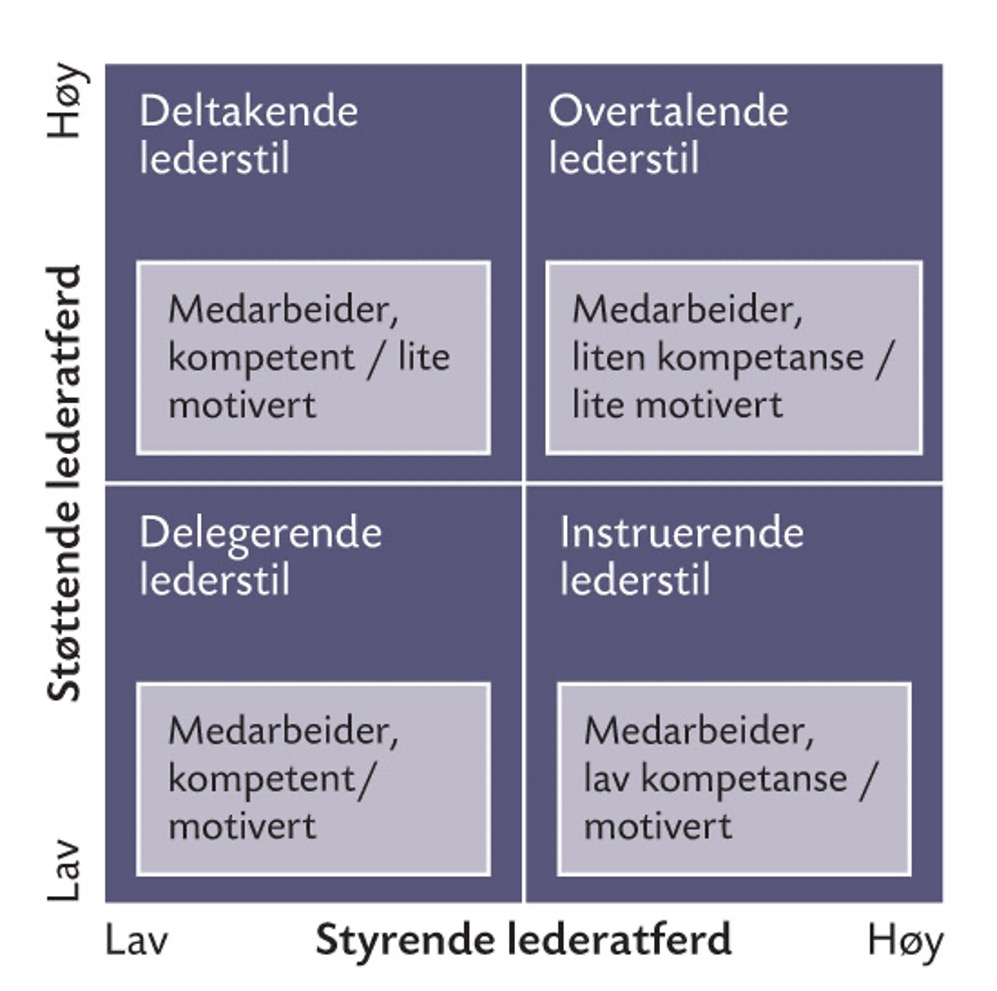
\includegraphics[width=8cm]{img/situasjonsbestemt.jpg}
  \caption{Situasjonsbestemt ledelse \parencite{ledelse}}
  \label{fig:situasjon}
\end{figure}

\emph{Situasjonsbestemt ledelse} går ut på å nettopp dette å tilpasse seg til situasjonen man er i. 
I Figur \ref{fig:situasjon} ser vi i hvilke situasjoner de ulike stilene faller til. 
Det første steget for en leder i møte med en quiet quitter er da å identifisere hvor i rubrikken medarbeideren faller, og tilpasse sin stil etter det. 

Felles for de fleste som driver med quiet quitting er motivasjonen. 
Det blir kanskje ikke nødvendig vis helt riktig å si at alle er lite motivert for arbeidet, men det vi med sikkerhet kan si er at de er svært lite motivert til å jobbe utover det de mener de er pliktig.
Med tanke på Figur \ref{fig:situasjon} blir det da riktig å si at de faller innenfor øvre del av tabellen.
Den andre aksen er ikke like lett å generalisere blant quiet quitters; holdningen deres reflekterer ikke nødvendig vis noe om hvilken kompetanse de har i feltet sitt. 
Noen kan være godt kompetente men ha et ønske om å ikke ta med seg arbeidet til middagsbordet, mens andre bare vil prøve å være anonyme og skjule at de har manglende kompetanse.
Da ser vi at lederen må være tilpasningsdyktig og enten deltakende og motiverende, eller overtalende og bestemt. 
Her er det også viktig å merke seg at med overtalende menes ikke autoritær og streng; det vil trolig bare forverre situasjonen.
En overtalende leder må klare å oppmuntre medarbeideren og være støttende arbeidet så de føler seg kompetente og verdsatt.
Det handler i stor grad om å kunne ha en god kommunikasjon og snakke \emph{med}, og ikke \emph{til} kollegaen.


\subsection{Hvordan leder man en Quiet quitter?}

Til nå har vi funnet ut hvordan ulike ledertyper kan oppleve en quiet quitter, og hvordan man skal håndtere å møte en. 
Men hva slags leder vil man, eller bør man være, hvis man vil være en god leder for en quiet quitter? 
Hvilken lederstil skal man sikte seg inn på?

For å finne ut hva man skal velge er det enkleste å først legge på bordet hva som trolig ikke vil fungere. 
Å være autoritær har allerede blitt nevnt, og det er nesten innlysende. 
En som ikke brenner for jobben og helst bare vil se på den som en nødvendighet for å få hjulene til å gå rundt, vil bare bli enda mindre motivert og inspirert hvis lederen oppleves krass, streng og urettferdig.
Denne må man klart styre unna.

Hva nå med <<\emph{La-det-skure}>>-lederen? 
Vi har allerede sett at denne lederen ikke var så engstelig for å jobbe med en quiet quitter, så kanskje det ligger en likesinnet kjærlighet mellom de? 
Trolig vil ikke noen av partene ha det vanskelig med hverandre, og kanskje til og med trives ganske godt i lag. 
For bedriftens del går det nok ikke derimot ikke like plettfritt.
En dårlig egnet leder, og ansatte som holder unna å gi det lille ekstra, klarer kanskje å holde en etablert bedrift flytende i gode tider, men det er nok kanskje også det beste de greier.

Den siste lederstilen jeg vil dra frem som kan være utfordrende i denne situasjonen er verdibasert ledelse; en stil som i de fleste andre tilfeller virkelig kan motivere ansatte. 
Problemet her er nok at ved å være en quiet quitter har man allerede innstilt seg på at jobben bare er en dyd av nødvendighet.
Å spille på bedriftens verdier og samfunnsoppdrag hjelper da ikke særlig mye, siden den ansatte har utstrålt at sine verdier handler mer om at de kan være fri, enn at bedriften får til det den trenger.
Denne er ikke et like dårlig valg som de to første, og kan i enkelte tilfeller, der alt den ansatte trenger bare er litt ekstra motivasjon, fungere, men den er nok ikke alltid en fulltreffer.

Men hva er det nå da som kan fungere? 
En ting man kan prøve er å akseptere <<byttehandelen>> medarbeideren inviterer til ved å definere og bli enige om veldig klare og presise arbeidsoppgaver.
På denne måten kan du som leder skape et sterkt tillitsbånd til medarbeideren som, så lenge det går begge veier, kan få medarbeideren til å føle mer frihet i arbeidet da de vet akkurat hva de skal gjøre og hva som forventes av dem. 
Dette blir en form for \emph{tillitsbasert ledelse} der du som leder viser at du har tillit til at medarbeideren skal og har riktig kompetanse til å gjøre det de skal. 
Medarbeideren blir mye mer selvstendig og får tillit til å lede seg selv, såkalt \emph{selvledelse}.
I beste fall kan man få ut av denne <<handelen>> at medarbeideren får mye mer engasjement i arbeidet, og viser interesse til å yte det lille ekstra. Denne byttehandelen eller <<transaksjonen>> kan vi kalle for \emph{transaksjonsledelse}.

Hvis man vil holde seg til litt mer tradisjonelle lederstiler, eller ikke har tilliten til at en radikal endring i ledelsen er riktig valg, kan \emph{transformasjonsledelse} være løsningen. 
Transformasjonsledelse bygger litt på det vi har vært innom tidligere og tar inn elementer fra både transaksjonsledelse og verdibasert ledelse, og kombinerer de på en slik måte at medarbeideren både får litt av friheten og byttehandelen fra transaksjonsledelsen samtidig som lederen prøver transformere eller omdanne medarbeiderens motivasjon gjennom virksomhetens visjoner og verdier. 
Dette kan være nøkkelen til å motivere og engasjere medarbeideren til å av og til gi det lille ekstra og yte litt mer, så lenge de ser at de får noe tilbake for all innsatsen. 
Men om det endrer innstillingen og drømmen til den ansatte om å gi slipp på arbeidets plikter, er bare opp til den ansatte.

Og kanskje var det nettopp det å gi slipp på arbeidets plikter som var Sinatras amerikanske drøm, <<\emph{Start spreading the news, I'm leaving today}>>. Alt han ville var å være fri å gjøre det han ville uten å engste seg over alle andre bekymringer, <<\emph{I want to be a part of it: New York, New York}>>.

\newpage
\section{Truer Quiet quitting organisasjonskulturen?}

Organisasjonskulturen, enkelt oppsummert til <<\emph{sånn gjør vi det her}>> mentaliteten \parencite{ledelse}, er en svært viktig del av en virksomhets verktøykasse for å skape samhold, et godt arbeidsmiljø og ivareta enkeltmennesker.
En god organisasjonskultur får også virksomheten til å skinne et godt lys utad, som gjør den attraktiv for kunder, samarbeidspartnere og nye ansatte.

\begin{figure}[H]
  \centering
  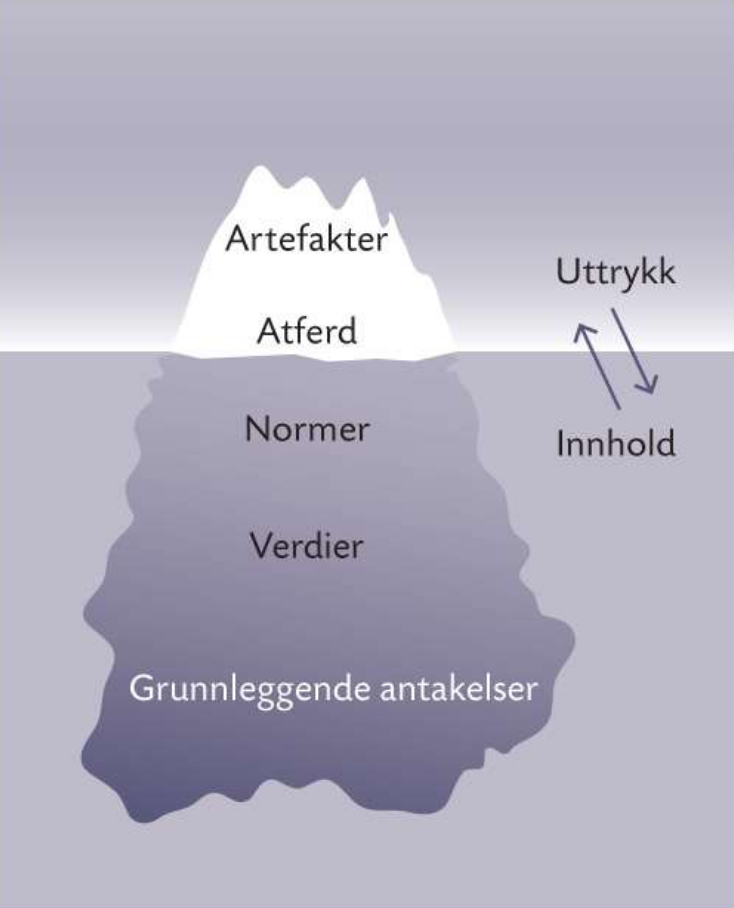
\includegraphics[width=7cm]{img/isfjell.png}
  \caption{Organisasjonskulturens isfjell \parencite{ledelse}}
  \label{fig:isfjell}
\end{figure}

Edgar H. Schein oppsummerte og beskrev hvordan organisasjonskulturen fungerer på tre nivåer med sitt metaforiske isfjell illustrert i Figur \ref{fig:isfjell}. 
Starter vi fra bunn av ser vi det som er hovedkilden og grunnsteinen i en virksomhets kultur, de \emph{grunnleggende antakelsene}. 
Disse tar de fleste for gitt, de diskuteres sjeldent, og kan ofte passere ubevisst for veldig mange.
Beveger vi oss opp et nivå finner vi virksomhetens \emph{normer og verdier}.
Disse kan oftere være oppe til diskusjon en de grunnleggende antakelsene, men vil sjeldent endres radikalt.
Normene og verdiene skal være med på å feste virksomhetens filosofi, vise hva de står for, og bidra til at alle arbeider mot et felles mål og visjon.
Øverst har vi virksomhetens \emph{atferd og artefakter}. Dette er utformende utrykk gjennom gjenstander og språk bygger virksomhetens merkevare, og viser den frem utad.
Her vil vi ofte finne slagord, logo, og til og med ansikter man man knytter til virksomheten; det folk flest assosierer og forbinder med virksomheten.

\subsection{Hva differensierer en Quiet quitter fra andre ansatte?}

En viktig del av å finne ut om quiet quitting kan true virksomheters organisasjonskultur er å markere forskjellene mellom en quiet quitter og dens medarbeidere.
Gitt premisset som blir fremstilt at <<\emph{I motsetning til quiet quitters er mange medarbeidere nemlig svært pliktoppfyllende og bidrar mye og gjerne ut over stillingsinstruksen}>>, kan vi tolke at en quiet quitter ikke er dette; de ønsker ikke å bidra med mer enn de må, og er ikke overflødig pliktoppfyllende.
Dette er den første ulikheten.

Den andre ulikheten finner vi i engasjementet de har til virksomheten. 
De fleste ansatte i en virksomhet vil gjerne gjøre et godt arbeid for virksomheten fordi de deler visjoner, verdier eller mål med virksomheten. 
Jo mer givende resultater man skaper er for en selv, desto mer ønsker man å bidra.
Det er ikke nødvendig vis slik at en quiet quitter ikke deler verdier eller visjoner med virksomheten, men personen har muligens ikke den samme brennende lidenskapen som en annen ansatt kan ha, og er mer opptatt av hva de kan oppnå personlig enn sammen med virksomheten.

\subsection{Skaper virksomheter Quiet quitters?}

Men hvor kommer interessen for quiet quitting fra?
Er det noe iboende hos enkelte mennesker som man bare må finne seg med, eller kan man ha blitt påvirket eksternt? 
Kommentator i Dagens Næringsliv Eva Grinde skriver om det hun mener er <<\emph{Bullshit-boomerangen som måtte komme}>> og inviterer leseren <<\emph{Velkommen til bullshitjungelen}>> \parencite{grinde22}.
Hun tar opp i sitt innlegg en ting hun mener, og håper, kan være <<\emph{en stille protest mot bortkastet tid, myter og bullshit som herjer arbeidslivet}>> \parencite{grinde22}.
Grinde hentyder at hun er lei av at bedrifter <<lyver>> om stillingsbeskrivelser som pynter og jazzer for mye på sannheten og kaller \emph{datasystemansvarlige} for \emph{virksomhetsarkitekter}, og \emph{renholdsarbeidere} for \emph{renholdskonsulenter}.
Og kanskje hun har et poeng, kanskje grunnen til at man velger å være en quiet quitter nettopp er å gjøre et lite opprør mot bedrifters trang til å pynte for mye med stillingstitler og kontrastere det med å vise hva de egentlig var ansatt for å gjøre?

Grinde peker også på at denne <<renessansen>> har blomstret etter pandemien.
I en tid der nesten alle landets arbeidsaktive jobbet hjemmefra, og satt i videomøter i pyjamasbuksa ved middagsbordet; den mentale avstanden mellom arbeid og fritid ble mye mindre. 
Mange ble dermed mye mer oppmerksom på hvor lett det var å <<bare svare på en mail før frokost>> eller <<se over gårsdagens referat mens klesvasken sto på>>,
og dermed også hvor vanskelig det kunne være å skape et klart skille mellom egentid og arbeidstid. 

For bedriftene er det like viktig at de ansatte har et sunt forhold til balansen mellom arbeid og fritid. For mye arbeidspress kan slite ut den ansatte, både fysisk og mentalt og gjøre at man presterer dårligere på jobb. <<\emph{Utbrenthet er blitt et velkjent fenomen og andelen av folk med psykiske problemer knyttet til jobben har økt gradvis de siste ti årene}>> forteller seniorforsker ved Statens arbeidsmiljøinstitutt Jan Olav Christensen til Bergens Tidene \parencite{bt22}.

Det kan virke som om quiet quitters vil kalle en spade for en spade, de vil ikke være <<løsningsarkitekter>> eller <<kommunikasjonskonsulenter>>. 
De vil gjøre den jobben de trengs til, og holde det der.

\subsection{Kan Quiet quitters være utfordrende for virksomheter?}

Til nå har vi sett at quiet quitting kontrasterer den tradisjonelle etablerte organisasjonskulturen i mange virksomheter; 
den som går ut på å motivere og engasjere medarbeiderne til å yte litt ekstra for å nå målene sine.
Det en virksomhet da må spørre seg selv er om den kan forvente å medregne at mange av de ansatte stadig skal gi av seg selv 110\%. 

I en virksomhet er det HR-avdelingen som skal ha ansvar å ta vare på de ansatte og passe på at de fungerer som den resursen virksomheten trenger, <<\emph{menneskelige ressurser}>> kalles HR tross alt på norsk. 
I en tid etter pandemien burde en virksomhet drevet med en smidig HR-avdeling plukke opp oppmerksomheten flere ansatte har lagt på balansegangen mellom arbeid og fritid, og stille opp som en støttespiller når man ser at ansatte begynner å bomme i sjongleringen mellom arbeid og fritid. 
En virksomhet som ikke håndterer å følge opp denne utviklingen kan i verste tilfelle ende opp med ansatte som mistrives på jobb og underleverer i arbeidet sitt.
Og det å måtte stadig sirkulere på ansatte koster mye mer både på økonomien, ressursene og omdømmet til en virksomhet.

Et annet punkt en HR-avdeling må være oppmerksom på er hvor mye tid de ansatte bruker uten om avtalt arbeidstid, både betalt og ubetalt. 
Hvis en ansatt bruker mye av egen tid til jobb-relatert arbeid kan det bli en stygg uvane som i verste fall kan føre til at den ansatte føler det ligger en forventning om at det er slik arbeidsforholdet skal være.
Hvis en virksomhet vil unngå å ha ansatte som viser tendenser til quiet quitting er dette en atferd man må se etter og reagere på raskt.
Det er viktig at den ansatte er klar over forventningene som legges til forventet arbeidsmengde og hvilke tider det skal utføres på.
Hvis de ansatte føler at de hele tiden må være tilgjengelige og ikke har en stilling som tilsier det, kan det rast føre dem i den første problemstillingen vi var innom.

\subsection{Skal man velge yrke etter lønn eller interesse?}

Det kan nå se ut som at quiet quitters i liten grad velger yrker etter interesse og motivasjon for arbeidet, så hva er det de går etter?
Man kan anta at det som hinderer noen i å bytte jobb er at de enten trives veldig godt med arbeidsoppgavene og arbeidsmiljøet, og/eller er fornøyd med lønne de tjener. 
Det å da anta at mange quiet quitters er relativt fornøyd med lønnen sin er ikke så urimelig. Spørsmålet blir da om det er riktig å velge et yrke kun ut ifra om man er fornøyd med lønnen, eller om man også må ha en interesse for arbeidet?

En ting man uansett må ha, i hvert fall for å bli ansatt, er riktig kompetanse til yrket.
En arbeidsgiver vil sjeldent ansette inkompetente medarbeidere, så gitt at man er kvalifisert skal ikke det være noe hinder for å få en jobb. 
Men hva da med interessen? 
Under en ansettelse, eller helst under intervjurunden, burde det komme frem om den potensielle arbeidstakeren har interesse for arbeidet eller ikke.
Det er da i praksis arbeidsgivers valg om å ansette personen på grunnlag av interessen og motivasjonen de viser.

Det er ikke derimot i alle tilfeller at arbeidsgiver har like stor valgmulighet.
I yrkesgrupper med mangel på arbeidskraft er markedet oftere styrt av arbeidstakeren, som da har større mulighet til å velge og vrake mellom jobbene.
Arbeidstakeren har da muligheten til å <<shoppe>> rundt og velge seg de stillingene som betaler mest, enten rent økonomisk eller med andre goder.
Tenker man da kynisk og antar at arbeidstakere alltid vil velge det som er best og enklest for dem, kan man potensielt finne flere som driver med quiet quitting i arbeidsmarkeder med høy etterspørsel.

I helt motsatt ende har vi de som opererer i overflødige marked; der tilbudet av arbeidskraft er langt høyere enn etterspørselen. 
Her vil kan vi tenke oss å finne færre som driver med quiet quitting fordi posisjonene er såpass utsatt at det å beholde jobben, og å vise at man er engasjert er viktig.
I Norge mister man heldigvis sjeldent jobben bare av å ikke være motivert nok, det skal tross alt litt til for å bli sagt opp. 
Men å underprestere i yrker med mange kvalifiserte kandidater bankende på døren kan gjøre at man enda fortere tviler på egen kompetanse, og vips har man havnet i en ond sirkel som sakte river på selvtilliten.

Konklusjonen blir da at enkelte virksomheter, gjerne de som virkelig skal bygge merkevaren sin og finne posisjonen sin, kan oppleve det vanskelig med quiet quitting.
Løsningen for disse vil da i mange tilfeller være å, så godt de kan, jobbe med de ansatte og føre en god kommunikasjon om hva man tenker som forventninger til arbeidsoppgaven.
Et sterkt og smidig HR-apparat vil gjøre denne jobben mye enklere og komfortabel for begge parter.
Men i enkelte tilfeller kan man ikke gjøre noe med personer som driver med quiet quitting, det handler rett og slett om hvor mye tid og energi den ansatte ønsker å vie til jobben sin;
noe mange ser på som en ren nødvendighet fremfor en lidenskap.
I disse tilfellene må virksomheten vurdere og enten bare akseptere at slik fungerer arbeidsmarkedet, eller så må de vurdere å endre sine egne verdier ut ifra hva de ansatte ønsker.

\newpage
\printbibliography[heading=bibintoc] % LAGER BIBLIOGRAFI

\end{document}
